\chapter{架构}

\section{RAID分析}

RAID分析作为架构驱动力

假设和信念
\begin{enumbox}
\item 云是新常态
\item 数据资产是战略资源
\item 全闪是大势所趋
\end{enumbox}

新设计解决了什么老问题?
\begin{enumbox}
\item 单卷的水平扩展问题
\item IO path上的数据转发问题
\item allocate性能低,影响精简配置和COW性能
\item 每个节点导出core、disk等资源,进行全局调度(均衡)
\item 灵活的MM
\item thread local影响CPU利用率
\item ***
\item 重新调整数据布局
\item 单卷大小的限制(支持大卷)
\item chkinfo是动态大小的,副本数、EC配置
\item 底层chunk对象依然不是跨卷的
\item ***
\item COW: volume和snapshot共享对象
\item ***
\item table1/table2实现过于复杂的问题
\item disk md and slots
\item coroutine难于调试
\item ***
\item 多网络
\item MULTIPATH
\item IPv6
\end{enumbox}

\section{模块}

分布式系统架构通常包括几个部分:client、mds、cds。分别对应什么?
\begin{center}
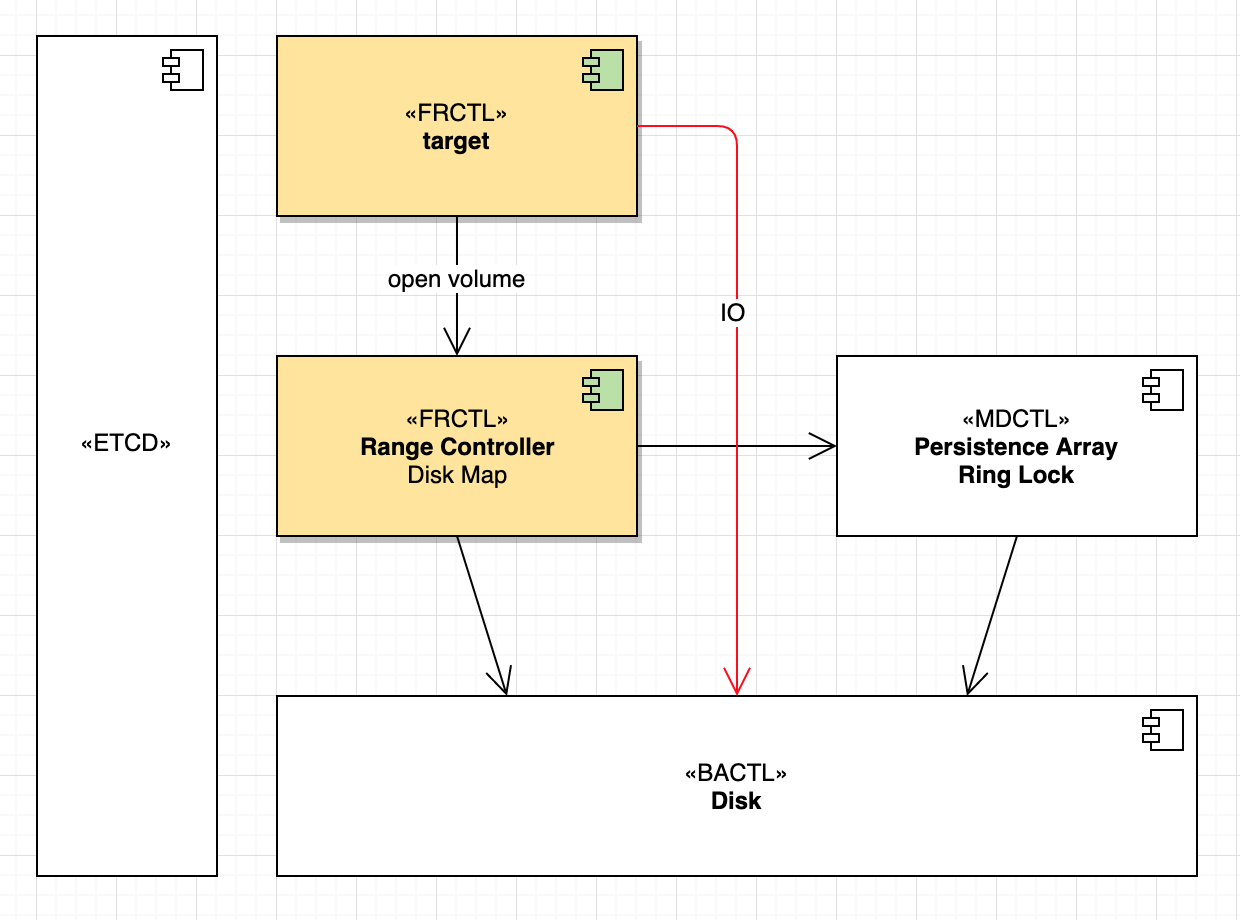
\includegraphics[width=11cm]{../imgs/modules.png}
\end{center}

target到bactl,有两条路径,视是否通过range ctl而定。如果不通过range ctl(rangectl bypass),数据流可直达后端存储,
实现控制流和数据流分流的目的。同时降低了转发成本。

问题集:
\begin{enumbox}
\item 为什么range ctl和mds是分离的进程?
\item vss是否必要?
\item ***
\item io路径是什么?
\item 副本一致性是如何实现的?
\item IO和Recovery之间如何同步?
\end{enumbox}

\subsection{FRCTL}

target如何与分布式卷相连?

vss包括4个range,range包括4个pa,pa包括固定数目的chunk。pa和chunk都是4M大小。
\todo{vss是否必要}vss是否必要,还是增加了设计复杂度?

token是向range ctl获取的,粒度为chunk。range ctl上每个chunk维护有token计数器。

token里包含了每个副本的位置信息,这是向mds请求得到的。

client并不与mds直接通信。分离fr和mds为两个进程,一是可以指定不同的core;二,便于debug。

\begin{center}
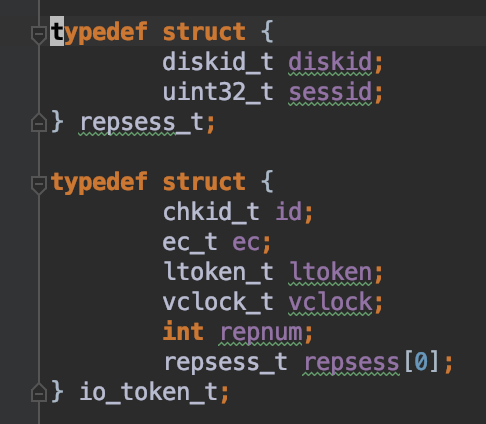
\includegraphics{../imgs/token.png}
\end{center}

range ctl和mds都在hash ring上。都采用了hash机制来定位目标节点。
所以\hl{有两个hash ring:range ctl和mds}。两个ring都通过mds master来维护。
ring的节点结构是什么?node and core?
\begin{center}
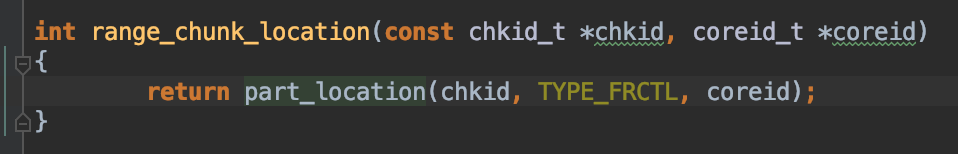
\includegraphics[width=11cm]{../imgs/chunk-location.png}
\end{center}

partition是range ctl和mdctl共用模块。range ctl目前归属frctl。

lease机制目前没用,如果需要把range ctl放置到session所在的位置(一个volume的所有range都在一个节点上?),
可以选用lease机制,而不用dht机制。怎么理解session?

一旦ring结构发生变化,会有什么影响?SSAN通过epoch来管理ring结构的变化。

ring上节点负载均匀性如何?

ring lock有什么用?在mds master上维护状态,处理ring发生变更的情况。
是否可通过引入epoch实现同样的功能?

GFM?解决全局同一视图的问题。

如何识别和处理stale消息?

\subsection{MDCTL}

hash ring上有一个节点充当master角色。如何选主,如何保持其唯一性?
通过etcd lock实现。

\subsection{BACTL}

diskid是全局的,在etcd上有目录。

\subsection{Driver}

diskmd磁盘访问接口,支持libnvme驱动。

需要管理物理内存,如hugepage和memory pool。

NVMe/RDMA需要访问物理内存。

\section{资源}

从\hl{资源的生命周期模型}开始思考。资源包括:\hl{集群、节点、core、磁盘、pool、volume、snapshot}等,以及内部资源。

ERD

\subsection{Cluster}

\subsection{Node}

Node是Process、Core、Disk等资源的合集。利用Core的方式是个亮点。

增删节点是重大事件

\subsection{Disk}

Disk导出,分配过程可以进行全局调度。

调度器位于md ctl。md ctl负责管理chkid到disk id的映射关系。
\todo{diskid类型}diskid采用16bit整数是否太小?

diskmap.c,不宜放入bactl。bactl所有API都带diskid,针对单盘进行。

怎么做到每个副本属于不同的节点的呢?

如何管理diskmap的版本呢?

\hl{数据分布的均匀性}: 节点和磁盘两种粒度

tier and cache?

负载均衡

\subsection{Pool}

\subsection{Volume}

\begin{enumbox}
\item TP
\item Recovery
\item Balance
\item QoS
\item ***
\item EC
\item Dedup
\item Compress
\item ***
\item RC
\end{enumbox}

\subsection{Snapshot}

如何共享底层对象?

consistency group

分析各种操作的复杂度,包括空间和时间。

\hrulefill

平安科技:可写快照

与COW平列实现ROW?

快照占据底层volume空间共享?

COW的问题
\begin{enumbox}
\item 影响写性能
\item Rollback慢
\item clone卷慢,scan snap tree。snapshot也可执行flatten
\end{enumbox}

snap头包含什么指针?

快照卷与物理卷什么对应关系,

映射表的管理粒度,是chunk还是page?范围,是全局还是私有?

COW一次读,两次写

ROW一次读,一次写

\hrulefill

SSAN的snapshot实现。

ROW,两层元数据?

vol id发生变化,凡是依赖于vol id的都需要进行适配。

\section{数据}

\subsection{ETCD}

\subsection{卷的元数据}

两层元数据,etcd指向顶层对象。每个对象属于一个卷,
因为不是一般的对象系统,\hl{在快照的情况下,无法直接共享}。
